% Options for packages loaded elsewhere
% Options for packages loaded elsewhere
\PassOptionsToPackage{unicode}{hyperref}
\PassOptionsToPackage{hyphens}{url}
\PassOptionsToPackage{dvipsnames,svgnames,x11names}{xcolor}
%
\documentclass[
  letterpaper,
  DIV=11,
  numbers=noendperiod]{scrartcl}
\usepackage{xcolor}
\usepackage{amsmath,amssymb}
\setcounter{secnumdepth}{-\maxdimen} % remove section numbering
\usepackage{iftex}
\ifPDFTeX
  \usepackage[T1]{fontenc}
  \usepackage[utf8]{inputenc}
  \usepackage{textcomp} % provide euro and other symbols
\else % if luatex or xetex
  \usepackage{unicode-math} % this also loads fontspec
  \defaultfontfeatures{Scale=MatchLowercase}
  \defaultfontfeatures[\rmfamily]{Ligatures=TeX,Scale=1}
\fi
\usepackage{lmodern}
\ifPDFTeX\else
  % xetex/luatex font selection
\fi
% Use upquote if available, for straight quotes in verbatim environments
\IfFileExists{upquote.sty}{\usepackage{upquote}}{}
\IfFileExists{microtype.sty}{% use microtype if available
  \usepackage[]{microtype}
  \UseMicrotypeSet[protrusion]{basicmath} % disable protrusion for tt fonts
}{}
\makeatletter
\@ifundefined{KOMAClassName}{% if non-KOMA class
  \IfFileExists{parskip.sty}{%
    \usepackage{parskip}
  }{% else
    \setlength{\parindent}{0pt}
    \setlength{\parskip}{6pt plus 2pt minus 1pt}}
}{% if KOMA class
  \KOMAoptions{parskip=half}}
\makeatother
% Make \paragraph and \subparagraph free-standing
\makeatletter
\ifx\paragraph\undefined\else
  \let\oldparagraph\paragraph
  \renewcommand{\paragraph}{
    \@ifstar
      \xxxParagraphStar
      \xxxParagraphNoStar
  }
  \newcommand{\xxxParagraphStar}[1]{\oldparagraph*{#1}\mbox{}}
  \newcommand{\xxxParagraphNoStar}[1]{\oldparagraph{#1}\mbox{}}
\fi
\ifx\subparagraph\undefined\else
  \let\oldsubparagraph\subparagraph
  \renewcommand{\subparagraph}{
    \@ifstar
      \xxxSubParagraphStar
      \xxxSubParagraphNoStar
  }
  \newcommand{\xxxSubParagraphStar}[1]{\oldsubparagraph*{#1}\mbox{}}
  \newcommand{\xxxSubParagraphNoStar}[1]{\oldsubparagraph{#1}\mbox{}}
\fi
\makeatother


\usepackage{longtable,booktabs,array}
\newcounter{none} % for unnumbered tables
\usepackage{calc} % for calculating minipage widths
% Correct order of tables after \paragraph or \subparagraph
\usepackage{etoolbox}
\makeatletter
\patchcmd\longtable{\par}{\if@noskipsec\mbox{}\fi\par}{}{}
\makeatother
% Allow footnotes in longtable head/foot
\IfFileExists{footnotehyper.sty}{\usepackage{footnotehyper}}{\usepackage{footnote}}
\makesavenoteenv{longtable}
\usepackage{graphicx}
\makeatletter
\newsavebox\pandoc@box
\newcommand*\pandocbounded[1]{% scales image to fit in text height/width
  \sbox\pandoc@box{#1}%
  \Gscale@div\@tempa{\textheight}{\dimexpr\ht\pandoc@box+\dp\pandoc@box\relax}%
  \Gscale@div\@tempb{\linewidth}{\wd\pandoc@box}%
  \ifdim\@tempb\p@<\@tempa\p@\let\@tempa\@tempb\fi% select the smaller of both
  \ifdim\@tempa\p@<\p@\scalebox{\@tempa}{\usebox\pandoc@box}%
  \else\usebox{\pandoc@box}%
  \fi%
}
% Set default figure placement to htbp
\def\fps@figure{htbp}
\makeatother





\setlength{\emergencystretch}{3em} % prevent overfull lines

\providecommand{\tightlist}{%
  \setlength{\itemsep}{0pt}\setlength{\parskip}{0pt}}



 


\KOMAoption{captions}{tableheading}
\makeatletter
\@ifpackageloaded{caption}{}{\usepackage{caption}}
\AtBeginDocument{%
\ifdefined\contentsname
  \renewcommand*\contentsname{Table of contents}
\else
  \newcommand\contentsname{Table of contents}
\fi
\ifdefined\listfigurename
  \renewcommand*\listfigurename{List of Figures}
\else
  \newcommand\listfigurename{List of Figures}
\fi
\ifdefined\listtablename
  \renewcommand*\listtablename{List of Tables}
\else
  \newcommand\listtablename{List of Tables}
\fi
\ifdefined\figurename
  \renewcommand*\figurename{Figure}
\else
  \newcommand\figurename{Figure}
\fi
\ifdefined\tablename
  \renewcommand*\tablename{Table}
\else
  \newcommand\tablename{Table}
\fi
}
\@ifpackageloaded{float}{}{\usepackage{float}}
\floatstyle{ruled}
\@ifundefined{c@chapter}{\newfloat{codelisting}{h}{lop}}{\newfloat{codelisting}{h}{lop}[chapter]}
\floatname{codelisting}{Listing}
\newcommand*\listoflistings{\listof{codelisting}{List of Listings}}
\makeatother
\makeatletter
\makeatother
\makeatletter
\@ifpackageloaded{caption}{}{\usepackage{caption}}
\@ifpackageloaded{subcaption}{}{\usepackage{subcaption}}
\makeatother
\usepackage{bookmark}
\IfFileExists{xurl.sty}{\usepackage{xurl}}{} % add URL line breaks if available
\urlstyle{same}
\hypersetup{
  pdftitle={The Impact of Personalized Marketing Spend on Customer Purchase Amount},
  pdfauthor={Jingye Li},
  colorlinks=true,
  linkcolor={blue},
  filecolor={Maroon},
  citecolor={Blue},
  urlcolor={Blue},
  pdfcreator={LaTeX via pandoc}}


\title{The Impact of Personalized Marketing Spend on Customer Purchase
Amount}
\author{Jingye Li}
\date{}
\begin{document}
\maketitle

\renewcommand*\contentsname{Table of contents}
{
\setcounter{tocdepth}{3}
\tableofcontents
}

\section{Introduction}\label{introduction}

This report analyzes the relationship between marketing expenditures and
customer purchase behavior in the previous quarter's personalized
campaign. Firms often allocate budget to ads, emails, and coupons to
drive sales, but the effectiveness of increased spending remains
unclear. Understanding whether higher spending translates to higher
purchases can optimize future marketing investments. This analysis uses
data to provide data-driven insights for budget decisions.

\section{Research Question}\label{research-question}

Does higher per-customer marketing spending lead to higher individual
purchase amounts? We specifically examine whether increased investment
in personalized marketing directly correlates with higher customer
purchase values across different customer segments.

\section{Dataset Introduction}\label{dataset-introduction}

The dataset contains customer-level records including marketing spend,
purchase amount, customer segment, and other campaign details. The
cleaning process removed missing values and invalid non-positive records
to ensure reliable analysis. Only complete and valid observations are
used.

\subsection{Dataset Description}\label{dataset-description}

The cleaned dataset contains 128observations and 4 variables. Variable
types include character (customer\_id, segment) and numeric
(marketing\_spend, purchase\_amount), which support the analysis of
marketing spend and purchase behavior.

\pandocbounded{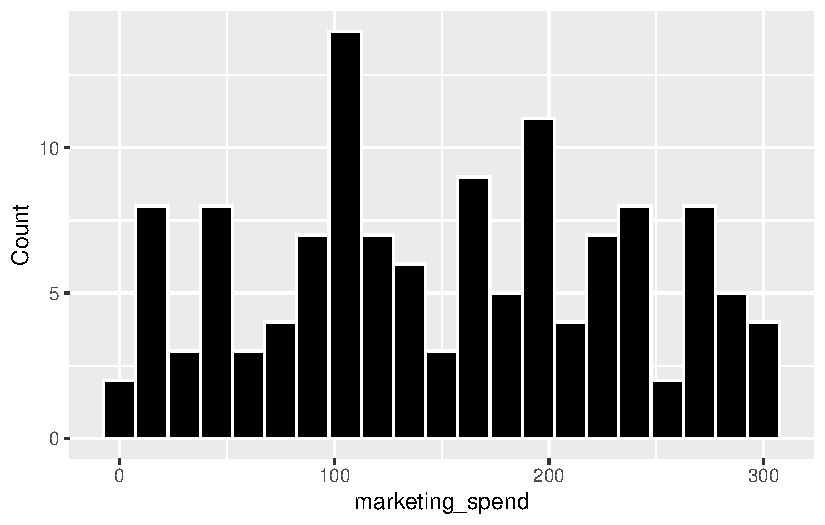
\includegraphics[keepaspectratio]{Untitled-1_files/figure-pdf/unnamed-chunk-2-1.pdf}}

The marketing expenditure ranges from 0 to 300 and is relatively evenly
distributed. This suggests that the marketing campaign covers a wide
range of spending levels, which helps ensure a more comprehensive
analysis of the relationship between marketing investment and revenue.

\begin{longtable}[]{@{}lll@{}}
\caption{Table 1: Summary Statistics of Key Numeric
Variables}\tabularnewline
\toprule\noalign{}
& marketing\_spend & purchase\_amount \\
\midrule\noalign{}
\endfirsthead
\toprule\noalign{}
& marketing\_spend & purchase\_amount \\
\midrule\noalign{}
\endhead
\bottomrule\noalign{}
\endlastfoot
& Min. : 1.36 & Min. : 3.28 \\
& 1st Qu.: 93.64 & 1st Qu.: 84.11 \\
& Median :153.84 & Median :157.28 \\
& Mean :152.05 & Mean :164.98 \\
& 3rd Qu.:223.83 & 3rd Qu.:241.81 \\
& Max. :299.85 & Max. :392.49 \\
\end{longtable}

This table shows descriptive statistics for marketing\_spend and
purchase\_amount, which helps understand the central tendency and spread
of the two key variables. \# Results section The research question asks
whether higher marketing spending leads to higher purchase amounts. To
answer this, two figures are created to visualize the relationship
between the key variables.

\begin{figure}[H]

{\centering \pandocbounded{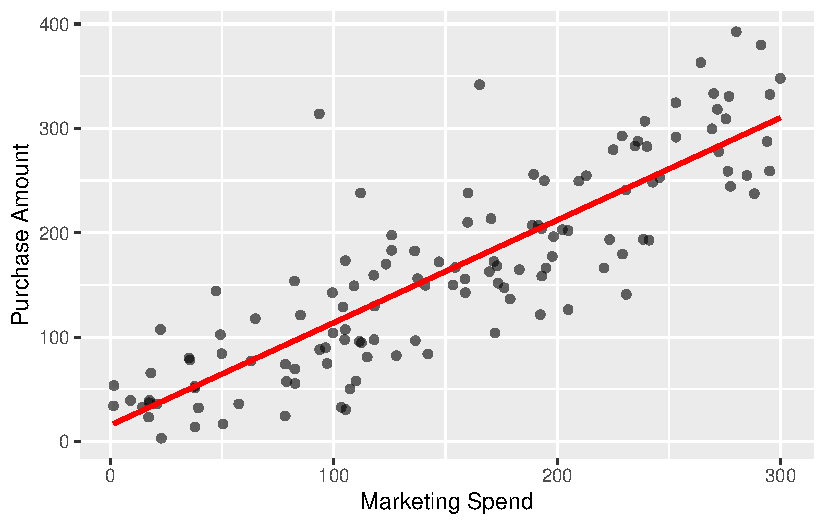
\includegraphics[keepaspectratio]{Untitled-1_files/figure-pdf/unnamed-chunk-4-1.pdf}}

}

\caption{Figure 1: Relationship between Marketing Spend and Purchase
Amount}

\end{figure}%

Figure 1 shows a clear positive linear relationship between marketing
spend and purchase amount. As marketing spend increases, purchase amount
tends to increase as well. The linear regression line confirms the
upward trend.

\begin{figure}[H]

{\centering \pandocbounded{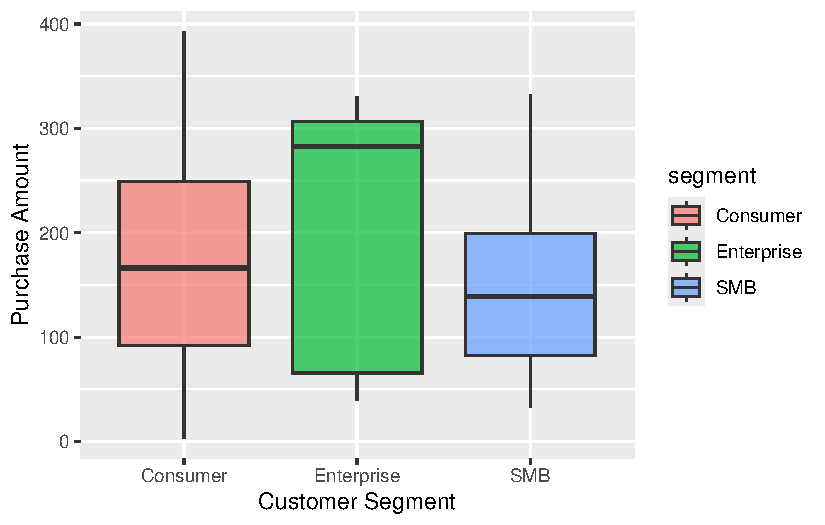
\includegraphics[keepaspectratio]{Untitled-1_files/figure-pdf/unnamed-chunk-5-1.pdf}}

}

\caption{Figure 2: Purchase Amount Distribution by Customer Segment}

\end{figure}%

Figure 2 shows the distribution of purchase amounts across the three
customer segments: Consumer, Enterprise, and SMB. Enterprise customers
have the highest median purchase amount, reaching approximately 280, and
the widest range of purchase values, with the largest box and extending
to nearly 340. In contrast, Consumer and SMB customers have lower and
more similar median purchase amounts, around 160 and 140 respectively,
with narrower value ranges. This indicates that while the overall
positive correlation between marketing spend and purchase amount holds
for all groups, Enterprise customers drive the highest purchase volumes
and show the greatest variability in spending behavior.

In summary, the visualizations clearly demonstrate a strong positive
relationship between marketing spend and purchase amount. As shown in
Figure 1, increased marketing spending is consistently associated with
higher purchase amounts, confirming a clear upward trend. Figure 2
further reveals that Enterprise customers generate the highest purchase
values, while Consumer and SMB customers show more stable spending
patterns. The average marketing spend for all customers is 152.05, and
the average purchase amount is 164.98. Together, these findings directly
answer the research question by providing strong evidence that higher
marketing spending leads to higher purchase amounts.




\end{document}
